\documentclass[12pt]{article}

\usepackage{physics}
\usepackage{siunitx}
\usepackage{enumerate}
\usepackage{graphicx}
\usepackage{caption}
\usepackage{csvsimple}

\begin{document}

    \title{Chord DHT Analysis Report}
    \author{Georgios Gkonis}
    \date{\today}

    \maketitle

    \begin{abstract}
        This report presents an analysis of a custom implementation of the Chord Distributed Hash Table (DHT) protocol.
        We explore the key operations of the protocol, benchmark their performance, and analyze the results using a dataset of computer scientists.
    \end{abstract}


    \section{Introduction}\label{sec:introduction}
    The Chord protocol is a scalable and distributed lookup protocol that can be used to locate the node responsible for a given key in a distributed system.
    This report analyzes four primary operations of the Chord DHT:
    \begin{itemize}
        \item Join: Adding a new node to the ring.
        \item Leave: Removing a node from the ring.
        \item Insert: Inserting a new key-value pair into the ring.
        \item Lookup: Searching for a key in the ring.
    \end{itemize}


    \section{Test Data}\label{sec:test-data}
    We utilized a dataset of computer scientists (scraped from Wikipedia) for testing the various operations of the Chord DHT implementation.
    The dataset includes:
    \begin{itemize}
        \item \texttt{name}: Last name of the scientist.
        \item \texttt{education}: Institution where the scientist received their first degree.
        \item \texttt{awards}: Number of awards received by the scientist.
    \end{itemize}


    \section{Benchmarking}\label{sec:benchmarking}
    We measured the time taken to perform each of the aforementioned operations for different sizes of the Chord ring.
    The results are discussed below.

    \subsection{Join Operation}\label{subsec:join-operation}
    The join operation involves adding a new node to the Chord ring.
    In our implementation, the node with the highest ID joins the ring, necessitating updates to the finger tables.

    \subsection{Leave Operation}\label{subsec:leave-operation}
    The leave operation consists of removing a node from the Chord ring.
    Here, we remove the node with the highest ID, which requires updating the finger tables of the remaining nodes.

    \subsection{Insertion Operation}\label{subsec:insertion-operation}
    The insertion operation adds a new key-value pair to the Chord ring.
    The node traverses its finger table to find the responsible node for the key, updating its own and other nodes' finger tables.

    \subsection{Lookup Operation}\label{subsec:lookup-operation}
    The lookup operation searches for a key in the Chord ring.
    The node traverses its finger table to locate the responsible node for the key.


    \section{Results}\label{sec:results}
    The average time taken to perform each operation for various sizes of the Chord ring is summarized in Table~\ref{tab:results}.
    The results are visualized in Figure~\ref{fig:benchmarks}.


    \begin{table}[h]
        \centering
        \csvautotabular{chord_dht_analysis.csv} % Load CSV data directly
        \caption{Average Time (ns) for Chord DHT Operations}
        \label{tab:results}
    \end{table}


    \begin{figure}[h]
        \centering
        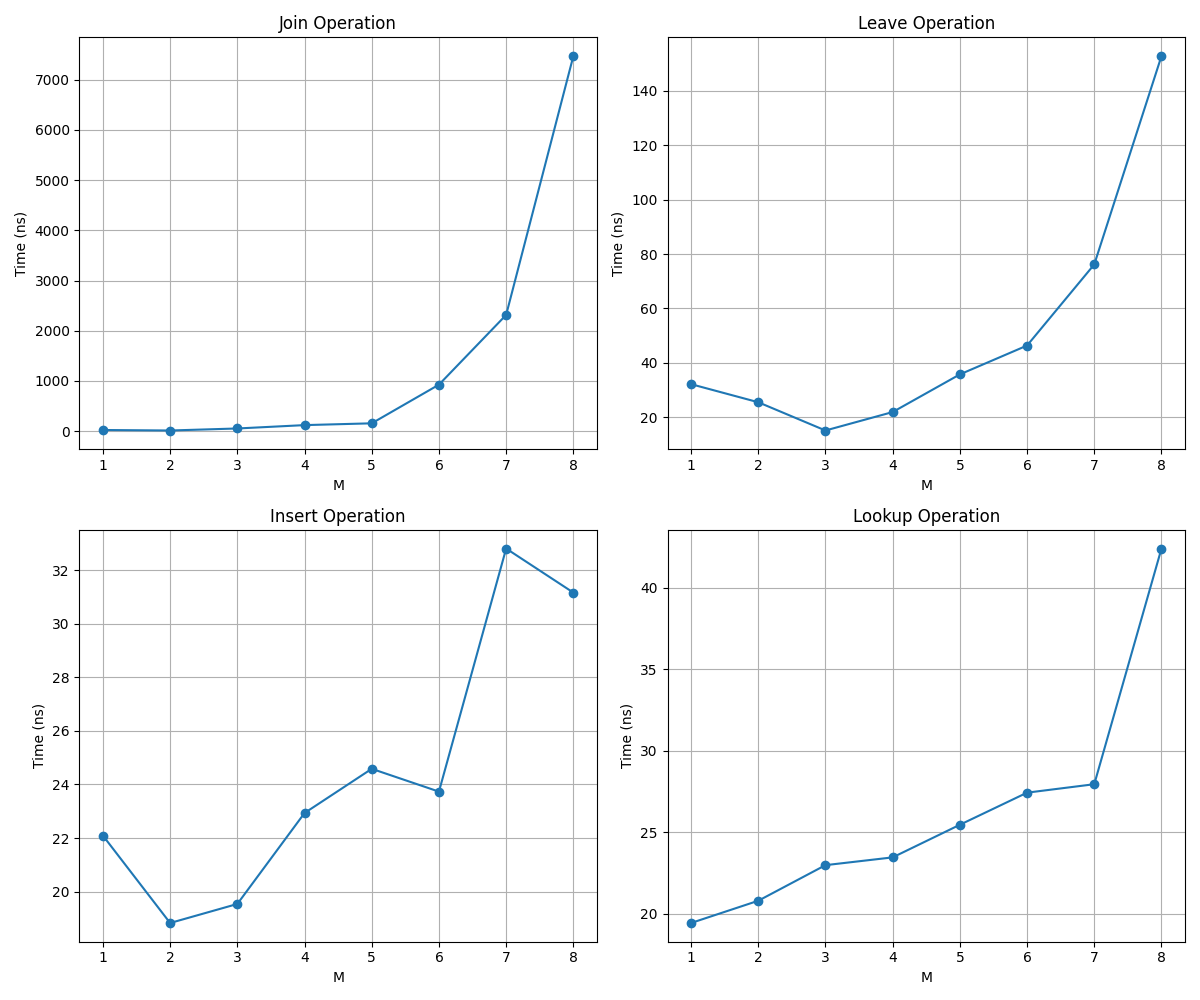
\includegraphics[width=0.8\textwidth]{chord_dht_analysis}
        \caption{Benchmark Results for Chord DHT Operations}
        \label{fig:benchmarks}
    \end{figure}

\end{document}
